% Tabela: Resultados do Experimento Delta
% \begin{figure*}[!ht]
\begin{table}[H]
	\centering
	\caption{Tabela de resultados do Experimento 1.}
		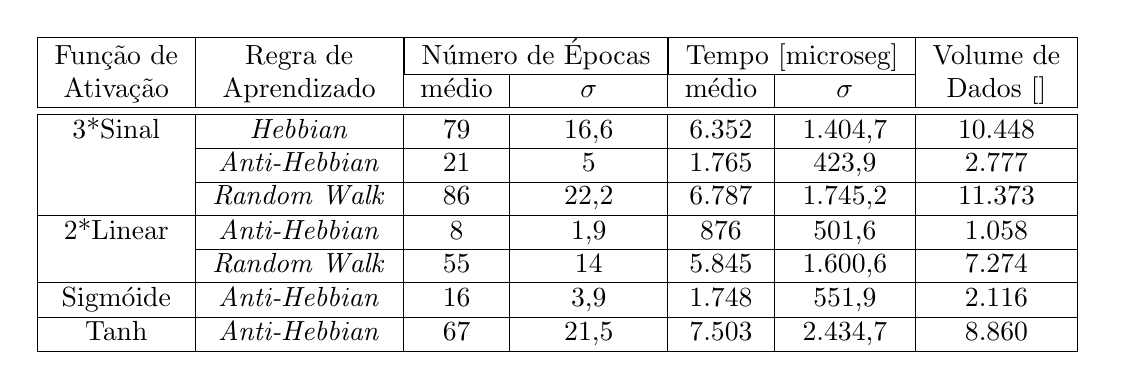
\begin{tikzpicture}
			
		\node[thick, align=center] (table) {
			\begin{tabular}{ |c|c|c|c|c|c|c| }
				\hline
				% \multicolumn{7}{ |c| }{Resultados do Experimento 1} \\
				% \hline \hline
				Função de &
				Regra de &
				\multicolumn{2}{ |c| }{Número de Épocas} &
				\multicolumn{2}{ |c| }{Tempo [microseg]} &
				Volume de \\ \cline{3-6}

				% Ativação & Aprendizado & mín & máx & médio & $\sigma$ & mín & máx & médio & $\sigma$ & Dados [\Bytes]\\
				Ativação & Aprendizado & médio & $\sigma$ & médio & $\sigma$ & Dados [\Bytes]\\
				\hline \hline
				
				% Signal
				\multirow{3}{*}{Sinal} & \textit{Hebbian} & 79 & 16,6 & 6.352 & 1.404,7 & 10.448 \\ \cline{2-7}
				& \textit{Anti-Hebbian} & 21 & 5 & 1.765 & 423,9 & 2.777 \\ \cline{2-7}
				& \textit{Random Walk} & 86 & 22,2 & 6.787 & 1.745,2 & 11.373 \\
				\hline

				% Linear
				\multirow{2}{*}{Linear} & \textit{Anti-Hebbian} & 8 & 1,9 & 876 & 501,6 & 1.058 \\ \cline{2-7}
				& \textit{Random Walk} & 55 & 14 & 5.845 & 1.600,6 & 7.274 \\
				\hline

				% Sigmoid
				Sigmóide & \textit{Anti-Hebbian} & 16 & 3,9 & 1.748 & 551,9 & 2.116 \\
				\hline

				% Hyperbolic Tangent
				Tanh & \textit{Anti-Hebbian} & 67 & 21,5 & 7.503 & 2.434,7 & 8.860 \\
				\hline
			\end{tabular}
		};

		\end{tikzpicture}
% 	\caption{Tabela de resultados do Experimento 1.}
	\label{tab:resultsDelta}
\end{table}